\chapter{Construction of 2D and 3D plots}
\section{Plotting functions}
Mathpar table allows you to build graphics ($tablePlot$), graphs of functions, which are explicitly defined ($plot$) or parametric ($paramPlot$).
You can build several different graphs in one coordinate system ($showPlots$).

Setting charting given command \comm{set2D}{()}.
If the command \comm{set2D}{()} has no parameters, the boundaries for the graphs are calculated automatically, and for explicit functions selected interval
$[0,1]$ along the horizontal axis. The names of the coordinate axes will be $X$ and $Y$, respectively. Title in the schedule will be absent.

If the command \comm{set2D}{()} user not asked, it is automatically set \comm{set2D}{()} with no arguments at the beginning of the session
the user.

There are 7 basic options of this command with the following parameters:
1) \comm{set2D}{()}\\
2) \comm{set2D}{(x0, x1)};\\
3) \comm{set2D}{(x0, x1, 'title')};\\
4) \comm{set2D}{(x0, x1, y0, y1)};\\
5) \comm{set2D}{(x0, x1, y0, y1, 'title')};\\
6) \comm{set2D}{(x0, x1, 'title', 'nameOX', 'nameOY')};\\
7) \comm{set2D}{(x0, x1, y0, y1, 'title', 'nameOX', 'nameOY')}.\\

Numbers $x0$ and $x1$ $(x0<x1)$ sets the interval along the axis of $OX$. Numbers $y0$ and $y1$ $(x0<x1)$ sets the interval along the axis of $OY$.
If these parameters are not specified, are calculated automatically. $nameOX$~--- signature on the axis $OX$, $nameOY$~--- signature on the axis $OY$, 
$title$~--- header graphics.

In addition, permitted to ask one or two keys that should be the last in the list of options: $BW$ and $ES$.
$BW$ refers to the construction of Cheraw and white graphics. $ES$ indicates equality zoom scale  $x$ axis ranges from $y$.
A total of $7*4=28$ different ways to set the parameters environment.

Character line which is depicted in the graph of each of the functions
$(plot, tablePlot, paramPlot)$ can be different: the solid line, dotted line, and the line that ends with an arrow.
To do this, these options are: '$dash$' (dotted line), '$arrow$' (arrows) and a combination of '$dashAndArrow$', which should be at the end of 
the parameter list of these functions.

For example, \comm{plot}{( x^2+1, 'dash')}.

If several separate graphs have names such as
P=\comm{plot}{(x^2)}; Q=\comm{tablePlot}{([[1,2], [3,4]])}; in this case they may be represented along with the command \comm{showPlots}{([P, Q])}.

The resulting plot can be downloaded from the site.
To do this, click on the button $\small \fbox{Download}$, which is located below the graph. The file is on schedule to be downloaded to your computer.


\subsection{Plots of explicit functions} 
To obtain the plot of an explicit function $f=f(x)$ the command 
\comm{plot}{(f)}.
Other options commands: \\
1) \comm{plot}{(f, [x0, x1])}, where $[x0, x1]$~--- interval along the axis of $OX$;\\
2) \comm{plot}{(f, [x0, x1], 'options')}, where $[x0, x1]$~--- interval along the axis of $OX$, 'options'~--- takes the following values:\\
1)'dash'~--- schedule will be a dashed line;\\ 
2)'arrow'~---  the last point on the graph is drawn with an arrow;\\
3)'dashAndArrow'~--- schedule will be a dashed line and the last point of the graph is drawn with an arrow.\\
3) \comm{plot}{(f, 'options')}. 
You can plot functions with parametric variables. The parametric variables are assigned when you set a environment (see ex.3). 

%begindelete
\underline{Example 1. }
%enddelete
\vspace*{-2mm}
\begin{verbatim}
SPACE = R64[x, y, z];
\set2D(-10, 10, -10, 10);
f = x^2 + \tg(x^2 - 1); 
p = \plot(f);
\end{verbatim}
\vspace*{-2mm}
%begindelete 


 
\ex{$f=x^2+\mathbf{tg}(x^2-1);$}{fig. \ref{301}.}


\begin{figure}[]
  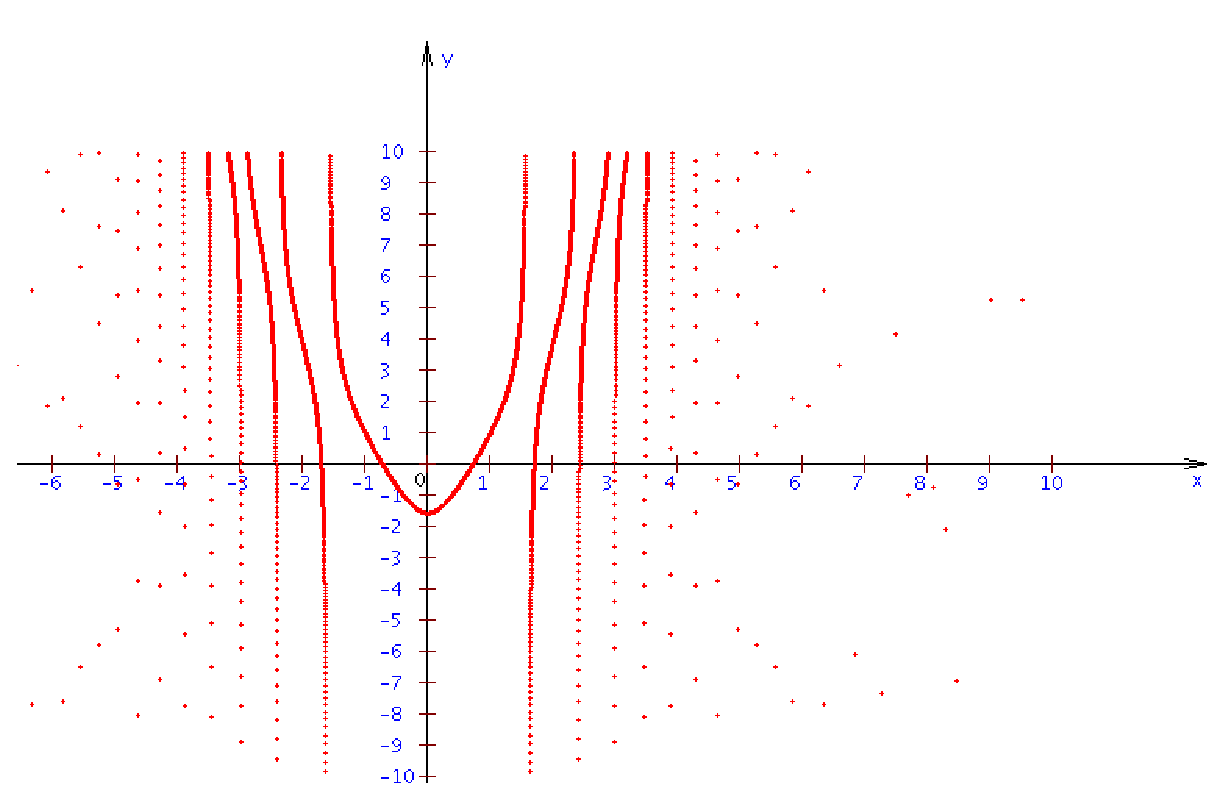
\includegraphics[scale=0.45]{pictures/3_1}
  \caption{ $f=x^2+\mathbf{tg}(x^2-1)$}
  \label{301}
\end{figure}

\eject
To get the graphs of several functions in one figure you must enclose the list 
of these functions in square brackets, as in the following example.

\underline{Example 2. }

%enddelete

\begin{verbatim}
SPACE = R64[x, y, z];
\set2D(-10, 10, -10, 10);
f = \sin(x); 
p = \plot([f, \tg(x)]);
\end{verbatim}
%begindelete

 \ex{$f=sin(x);$}{fig. \ref{3_3}. }

\begin{figure}[!h]
  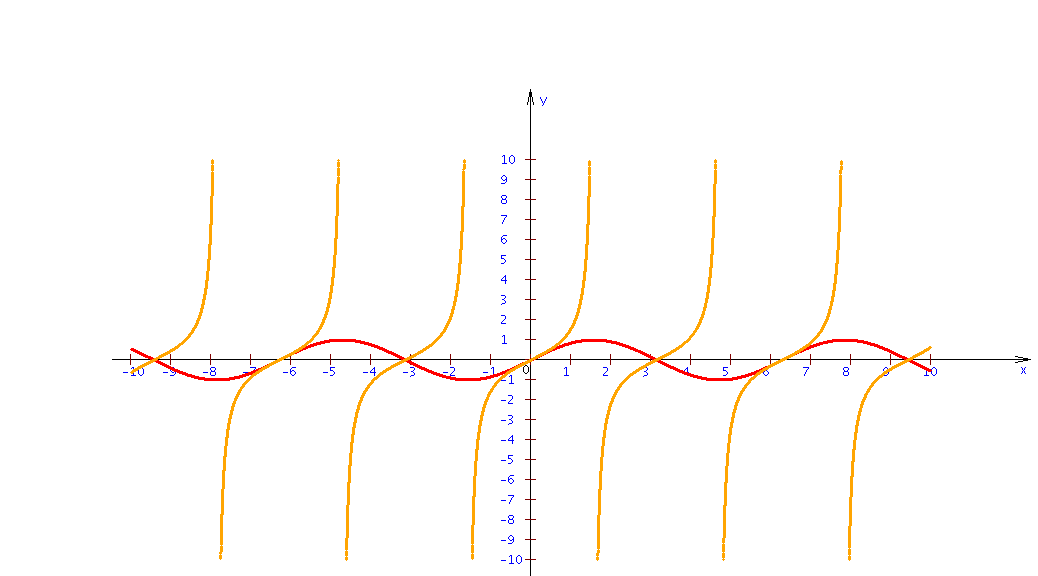
\includegraphics[width=274.6pt,height=152.38pt]{pictures/3_3}
  \caption{ $f = \sin(x)$ and $g = \mathbf{tg}(x)$}
  \label{3_3}
\end{figure}

\underline{Example 3. }

%enddelete

\begin{verbatim}
SPACE = R64[x, y, z];
\set2D(-10, 10, 0, 2);
f = \unitBox(x,3); 
p = \plot(f);
\end{verbatim}
%begindelete

%\ex{$f=unitBox(x,3);$}{fig. \ref{3_3}. }

%\begin{figure}[!h]
%  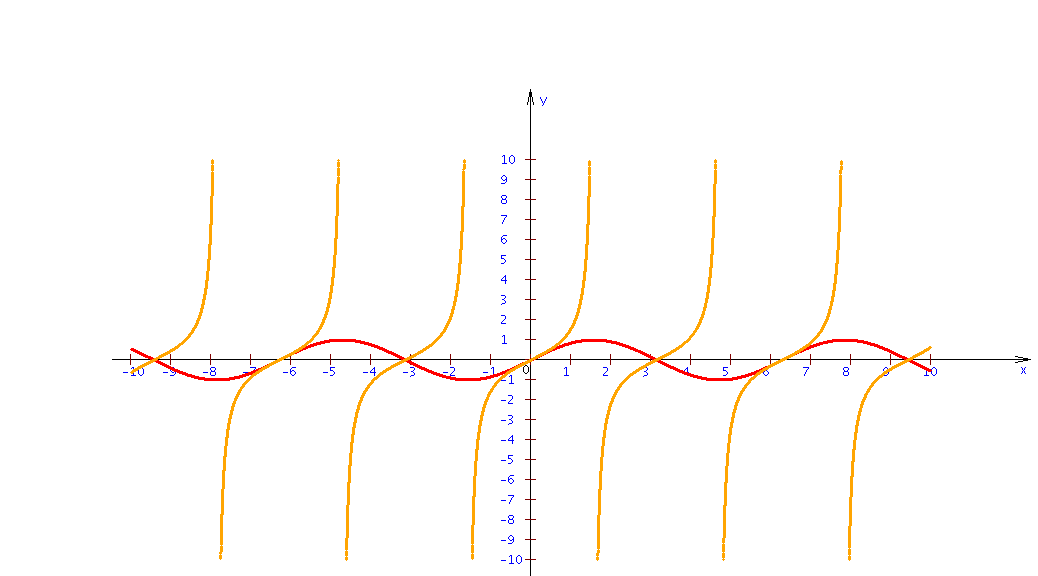
\includegraphics[width=274.6pt,height=152.38pt]{pictures/3_3}
%  \caption{ $f = \sin(x)$ и $g = \tg(x)$}
%  \label{3_3}
%\end{figure}


\underline{Example 4. }

%enddelete

\begin{verbatim}
SPACE = R64[x, a, b, c];
\set2D(0, 2\pi, 0, 2);
\plot(a\sin(bx) + c);
\end{verbatim}

%begindelete

%  \ex{$f=sin(x);$}{pict. \ref{3_3}. }
% 
% \begin{figure}[!h]
%   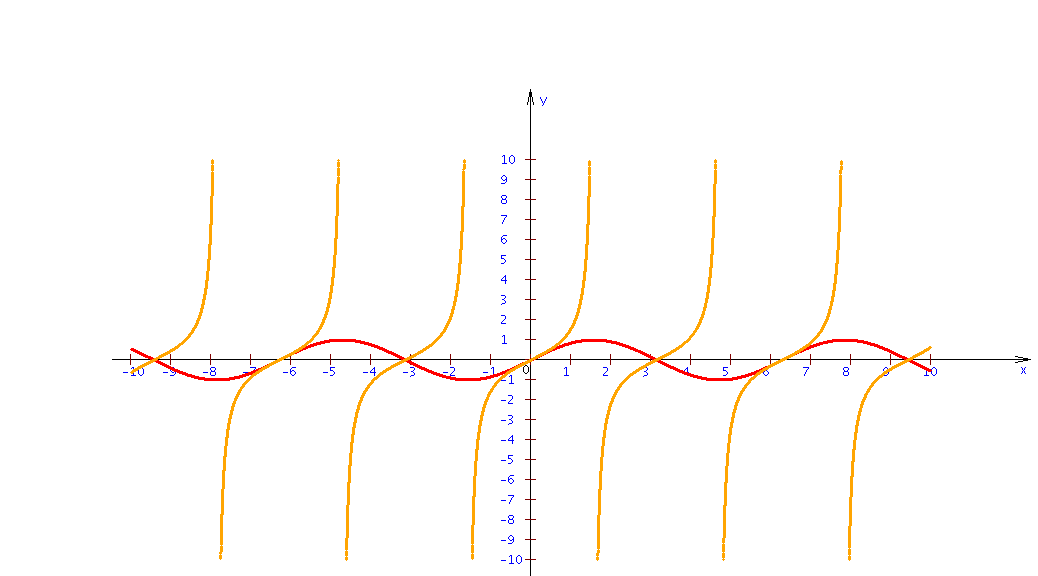
\includegraphics[width=274.6pt,height=152.38pt]{pictures/3_3}
%   \caption{Графики функций $f = \sin(x)$ и $g = \tg(x)$}
%   \label{3_3}
% \end{figure}
%enddelete

%begindelete
\underline{Example 5. }
%enddelete
\vspace*{-2mm}
\begin{verbatim}
SPACE = R64[x, y, z];
\set2D(-10, 10, -10, 10,'a','b','title');
f = x^2; 
p = \plot(f);
\end{verbatim}
\vspace*{-2mm}

%begindelete
\underline{Example 6. }
%enddelete
\vspace*{-2mm}
\begin{verbatim}
SPACE = R64[x, y, z];
\set2D(-10, 10, -10, 10);
f = x; 
p = \plot(f,'dash');
\end{verbatim}
\vspace*{-2mm}

%begindelete
\underline{Example 7. }
%enddelete
\vspace*{-2mm}
\begin{verbatim}
SPACE = R64[x, y, z]; 
f = x; 
p = \plot(f,[-5,5],'arrow');
\end{verbatim}
\vspace*{-2mm}

%begindelete
\underline{Example 8. }
%enddelete
\vspace*{-2mm}
\begin{verbatim}
SPACE = R64[x, y, z]; 
\set2D(-10, 10, -10, 10);
\plot([x,-x],'arrow');
\end{verbatim}
\vspace*{-2mm}
 
\subsection{Plots of parametric functions}  
To obtain the plot of parametric function \{$f=x(t)$, $g=y(t)$\} the command 
\comm{paramPlot}{([f, g], [t0, t1])} is used, where $[t0, t1]$ is an interval of variation of $t$.
Another version of the command:  \comm{paramPlot}{([f, g], [t0, t1], 'options')}, where $[t0, t1]$~--- the range of values for the parameter change, 
'options'~---  the following values:\\
1)'dash'~--- schedule will be a dashed line;\\ 
2)'arrow'~---  the last point on the graph is drawn with an arrow;\\
3)'dashAndArrow'~--- schedule will be a dashed line and the last point of the graph is drawn with an arrow.\\

%begindelete

\underline{Example 1. }


\nopagebreak
%enddelete
\vspace*{-2mm}
\begin{verbatim}
SPACE = R64[x, y, z];
g = \sin(x); 
k = \cos(x); 
f = \paramPlot([g, k], [0, 2\pi]);
\end{verbatim}
\vspace*{-2mm}

%begindelete
\ex{$g=sin(x); k=cos(x);$}{fig. \ref{3_4}.}
\begin{figure}[h!]
 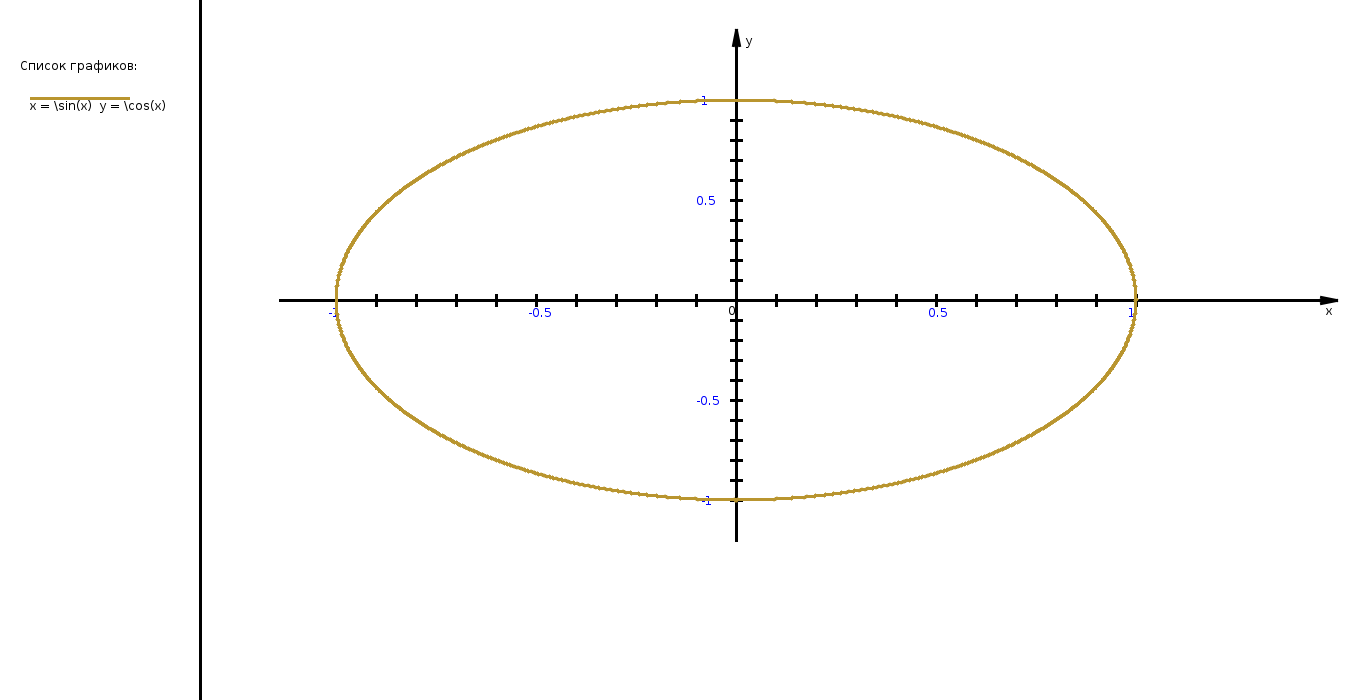
\includegraphics[scale=0.26]{pictures/2_1}
\vspace*{-10mm}
\caption{}
\label{3_4}
\end{figure}
%enddelete


%begindelete
\eject
\underline{Example 2. }


%enddelete
\vspace*{-2mm}
\begin{verbatim}
SPACE = R64[x, y, z];
g = x\sin(x);
k = x\cos(x);
f = \paramPlot([g, k], [0, 5\pi]);
\end{verbatim}
\vspace*{-2mm}

%begindelete
\ex{$g=x\sin(x); k=x\cos(x);$}{fig. \ref{2_2}.}
\begin{figure}[h!]
 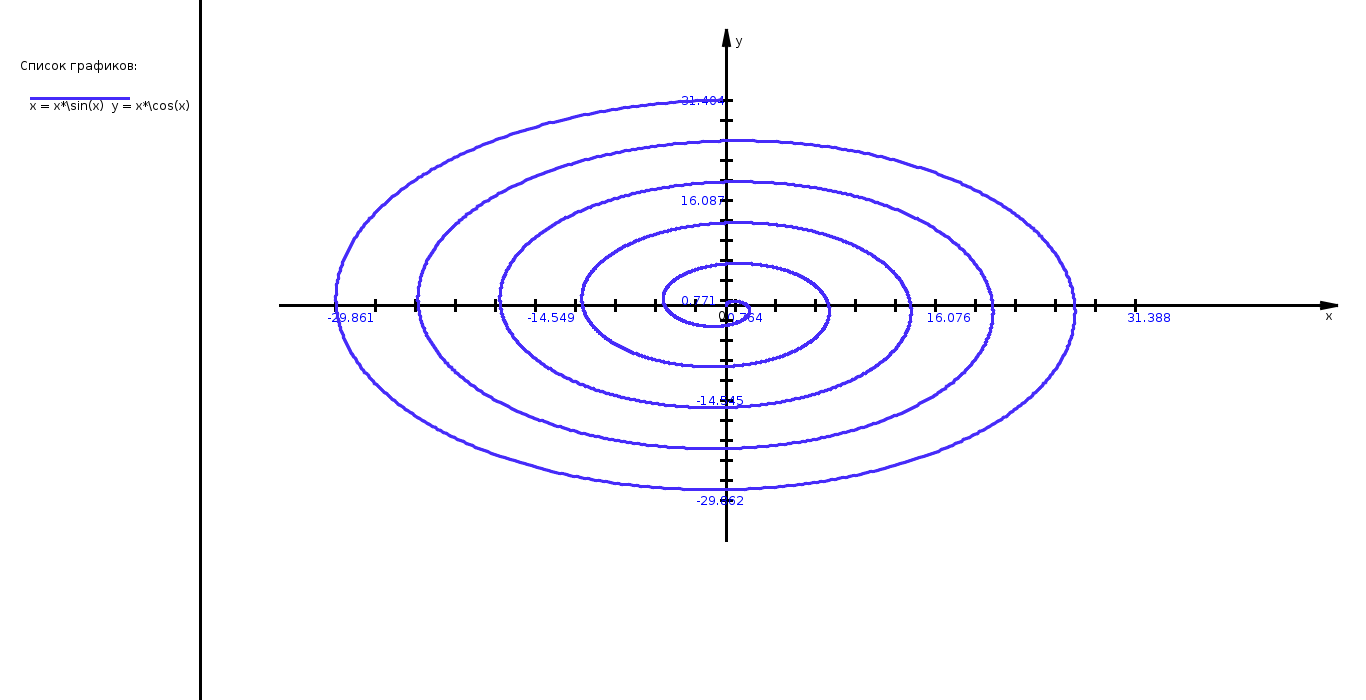
\includegraphics[scale=0.3]{pictures/2_2}
\vspace*{-10mm}
\caption{}
\label{2_2}
\end{figure}



\underline{Example 3. }

%enddelete

\vspace*{-2mm}
\begin{verbatim}
SPACE = R64[x, y, z];
g = 2\cos(x)+\cos(2x); 
k = 2\sin(x)-\sin(2x);
f = \paramPlot([g, k], [0, 2\pi]);
\end{verbatim}
\vspace*{-2mm}

%begindelete
\ex{$g=2\cos(x)+\cos(2x); k= 2\sin(x)-\sin(2x);$}{fig. \ref{2_3}.}
\begin{figure}[h!]
 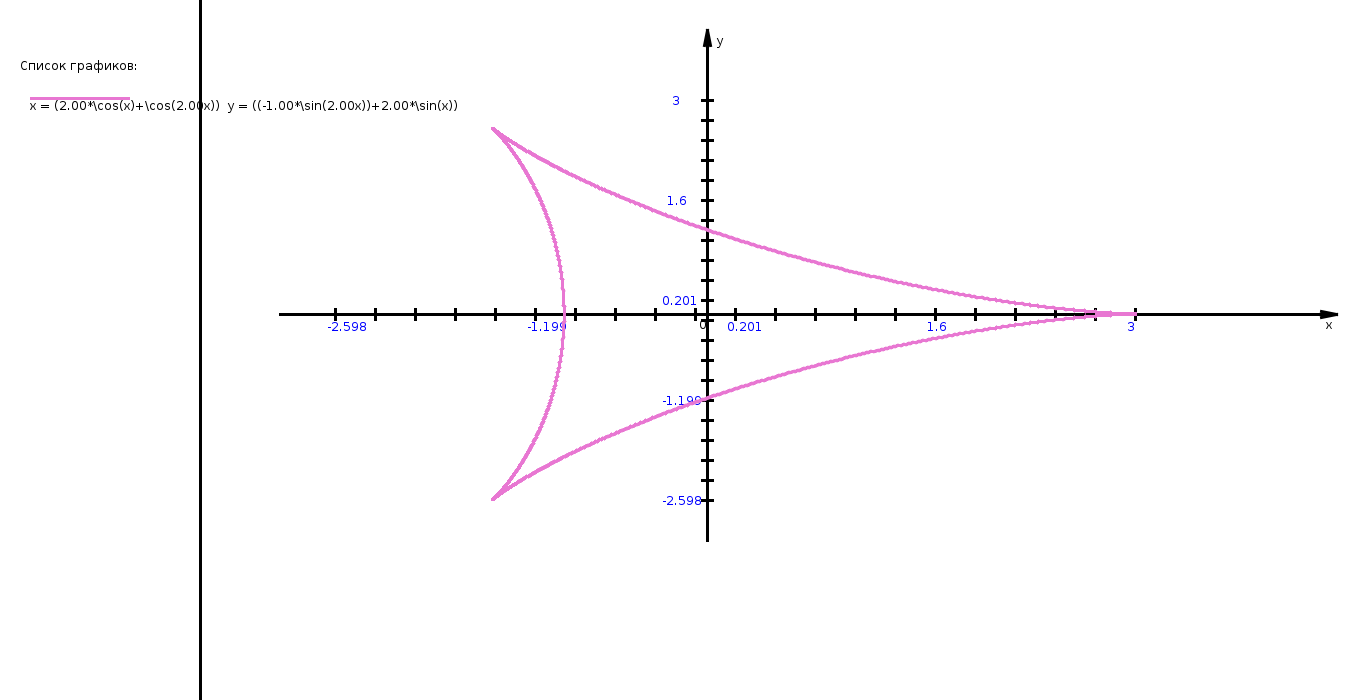
\includegraphics[scale=0.3]{pictures/2_3}
\vspace*{-10mm}
\caption{}
\label{2_3}
\end{figure}

\eject
\underline{Example 4. }


%enddelete

\vspace*{-2mm}
\begin{verbatim}
SPACE = R64[x, y, z];
g = 2\sin(x)^3; 
k = 2\cos(x)^3;
f = \paramPlot([g, k], [0, 2\pi]);
\end{verbatim}
\vspace*{-2mm}


%begindelete
\ex{$g=2\sin(x)^3; k= 2\cos^3(x)$}{fig. \ref{2_4}.}
\begin{figure}[h!]
 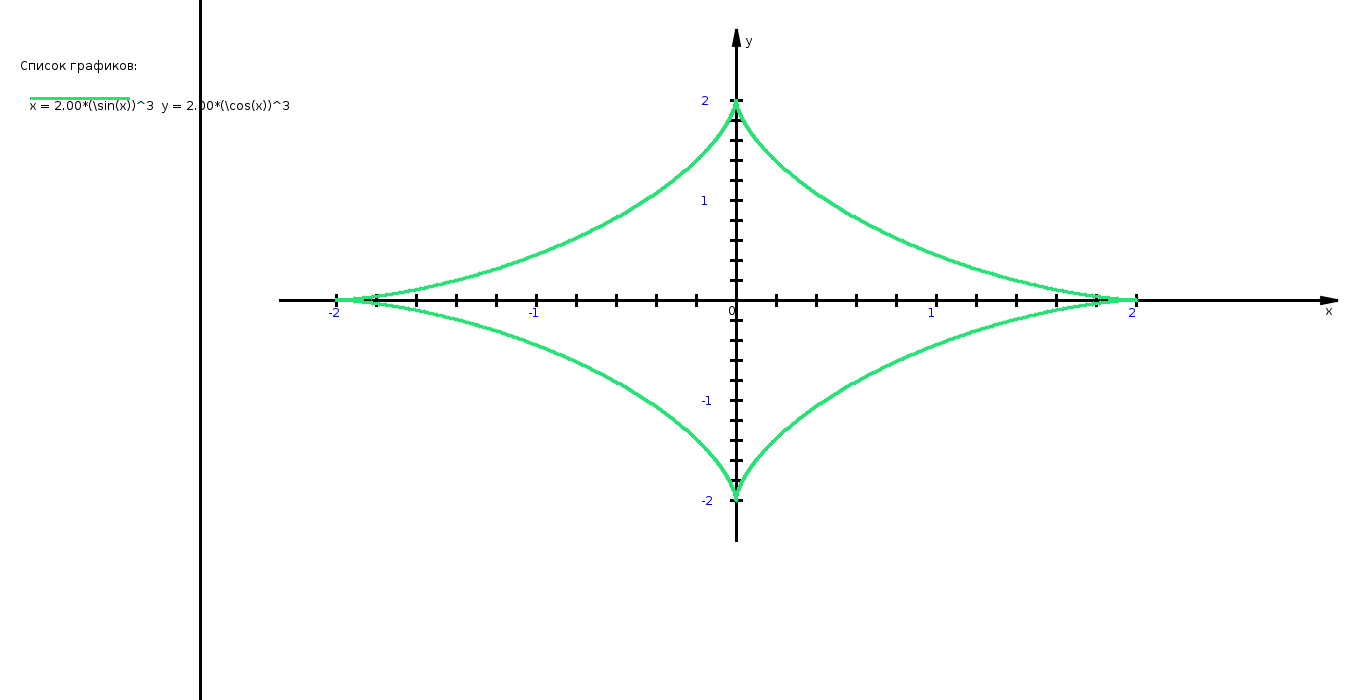
\includegraphics[scale=0.3]{pictures/2_4}
\vspace*{-10mm}
\caption{}
\label{2_4}
\end{figure}



\underline{Example 5. }
%enddelete

\vspace*{-2mm}
\begin{verbatim}
SPACE = R64[x, y, z];
g = (1+\cos(x))\cos(x); 
k = (1+\cos(x))\sin(x);
f = \paramPlot([g, k], [0, 2\pi]);
\end{verbatim}
\vspace*{-2mm}

%begindelete
\ex{$g=(1+\cos(x))\cos(x);k= (1+\cos(x))\sin(x);$}{fig. \ref{2_5}.}
\begin{figure}[h!]
 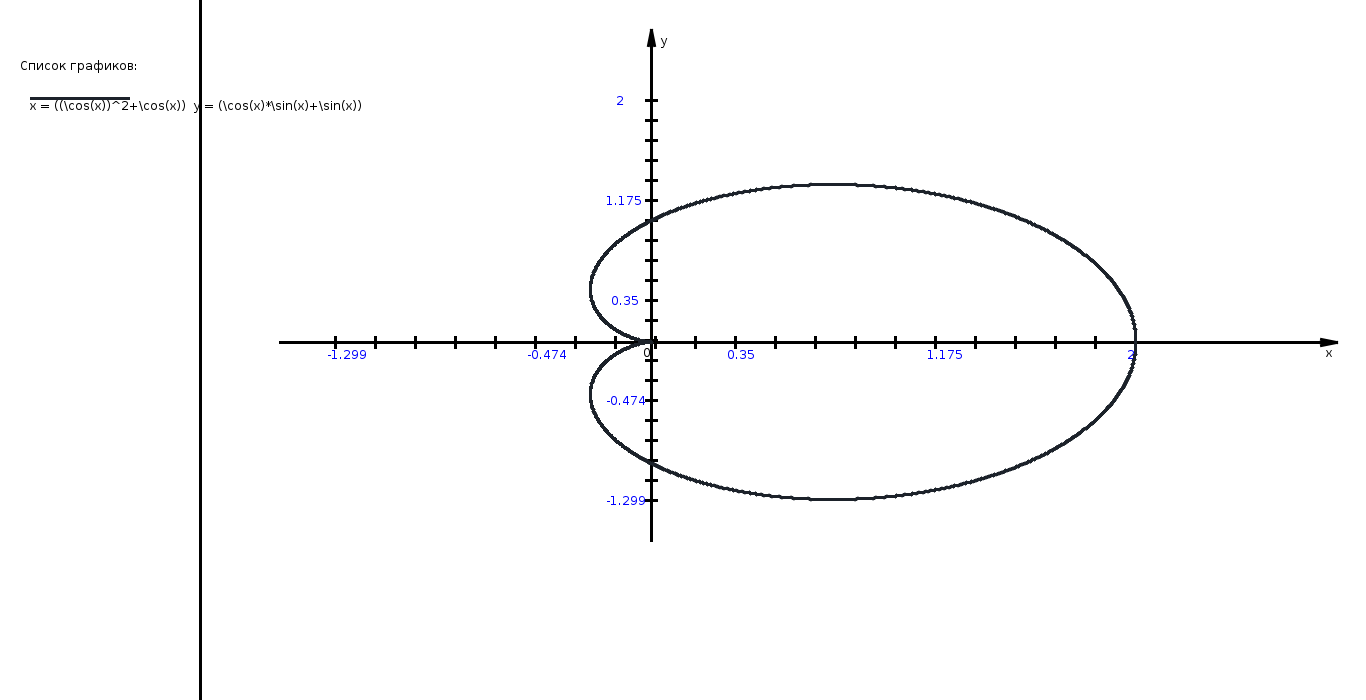
\includegraphics[scale=0.3]{pictures/2_5}
\vspace*{-10mm}
\caption{}
\label{2_5}
\end{figure}

%begindelete
\eject
\underline{Example 6. }
%enddelete


\vspace*{-2mm}
\begin{verbatim}
SPACE = R64[x, y, z];
g = \sin(x)(\exp(\cos(x))-2\cos(4x)+\sin(x/12)^5);
k = \cos(x)(\exp(\cos(x))-2\cos(4x)+\sin(x/12)^5);
f = \paramPlot([g, k], [0, 12\pi]);
\end{verbatim}
\vspace*{-2mm}


%begindelete
\ex{$g=\sin(x)(\exp(\cos(x))-2\cos(4x)+\sin^5(x/12));$\\
\hspace*{4mm} $k= \cos(x)(\exp(\cos(x))-2\cos(4x)+\sin^5(x/12));$}{fig. \ref{2_6}.}
\begin{figure}[h!]
 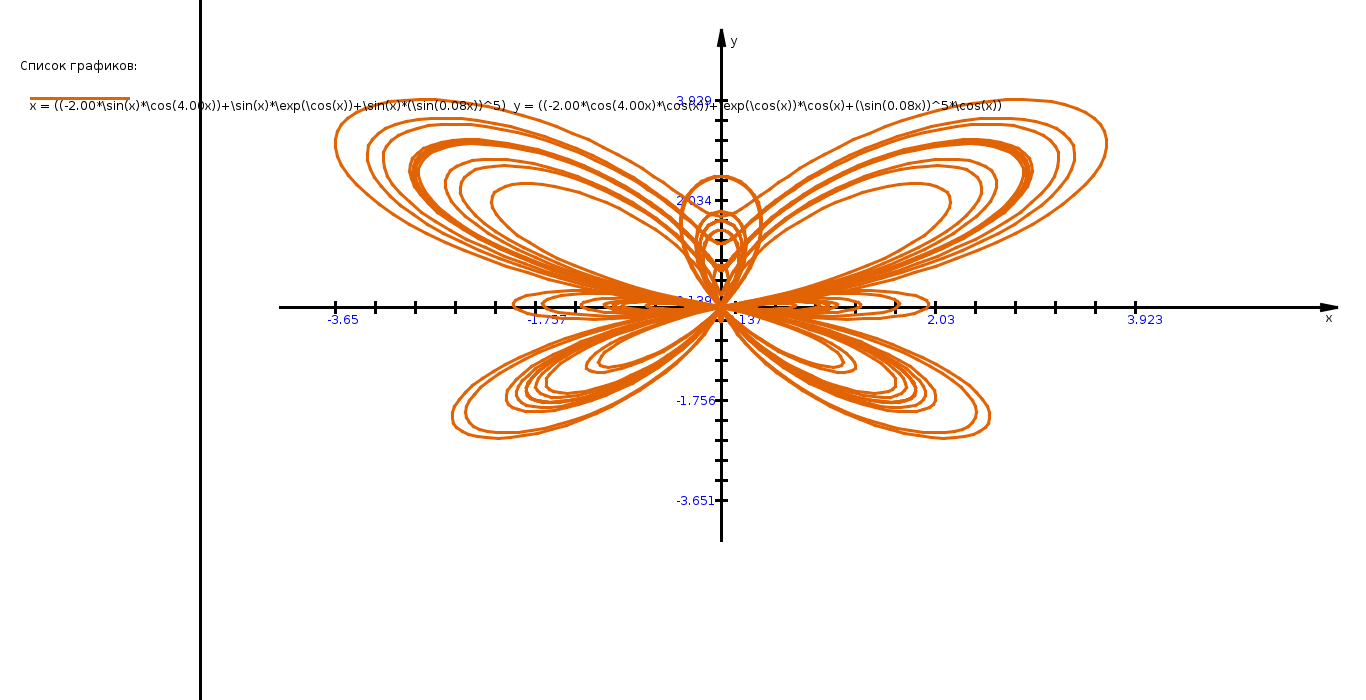
\includegraphics[scale=0.3]{pictures/2_6}
\vspace*{-10mm}
\caption{}
\label{2_6}
\end{figure}


\eject
\underline{Example 7. }
%enddelete


\vspace*{-2mm}
\begin{verbatim}
SPACE = R64[x, y, z];
\set2D('','','','','x(t)','y(t)','paramPlot');
g = \sin(x)(\exp(\cos(x))-2\cos(4x)+\sin(x/12)^5);
k = \cos(x)(\exp(\cos(x))-2\cos(4x)+\sin(x/12)^5);
f = \paramPlot([g, k], [0, 12\pi]);
\end{verbatim}
\vspace*{-2mm}

%begindelete
\eject
\underline{Example 8. }
%enddelete

\vspace*{-2mm}
\begin{verbatim}
SPACE = R64[x, y, z];
g = \sin(x); 
k = \cos(x); 
f = \paramPlot([g, k], [0, 2\pi],'dashAndArrow');
\end{verbatim}
\vspace*{-2mm}

\subsection{Plot of table function} 
To plot a function, which is defined by the table of points you have to execute the command: 
\comm{tablePlot}{([[x_{1},\ldots, x_{n}],[y_{11},\ldots,a_{1n}],\ldots,[y_{k1},\ldots,a_{kn}]])}.\\
Another version of the command:
\comm{tablePlot}{([[x_{1},\ldots, x_{n}],[y_{11},\ldots,a_{1n}],\ldots,[y_{k1},\ldots,a_{kn}]], 'options')}
,where 'options'~--- the following values:\\
1)'dash'~--- schedule will be a dashed line;\\ 
2)'arrow'~---  the last point on the graph is drawn with an arrow;\\
3)'dashAndArrow'~--- schedule will be a dashed line and the last point of the graph is drawn with an arrow.

%begindelete
\underline{Example 1.}
 
 \vspace*{-2mm}
%enddelete

 \begin{verbatim}
SPACE = R64[x, y, z];
 \tablePlot(
   [
     [0, 1, 2, 3, 4, 5],
     [0, 1, 4, 9, 16, 25],
     [0, -1, -2, -3, -4, -5],
     [0, 4, 8, 12, 16, 20]
   ]);
 \end{verbatim}

 %begindelete
\ex{}{fig. \ref{2_7}.}
\begin{figure}[!h]
 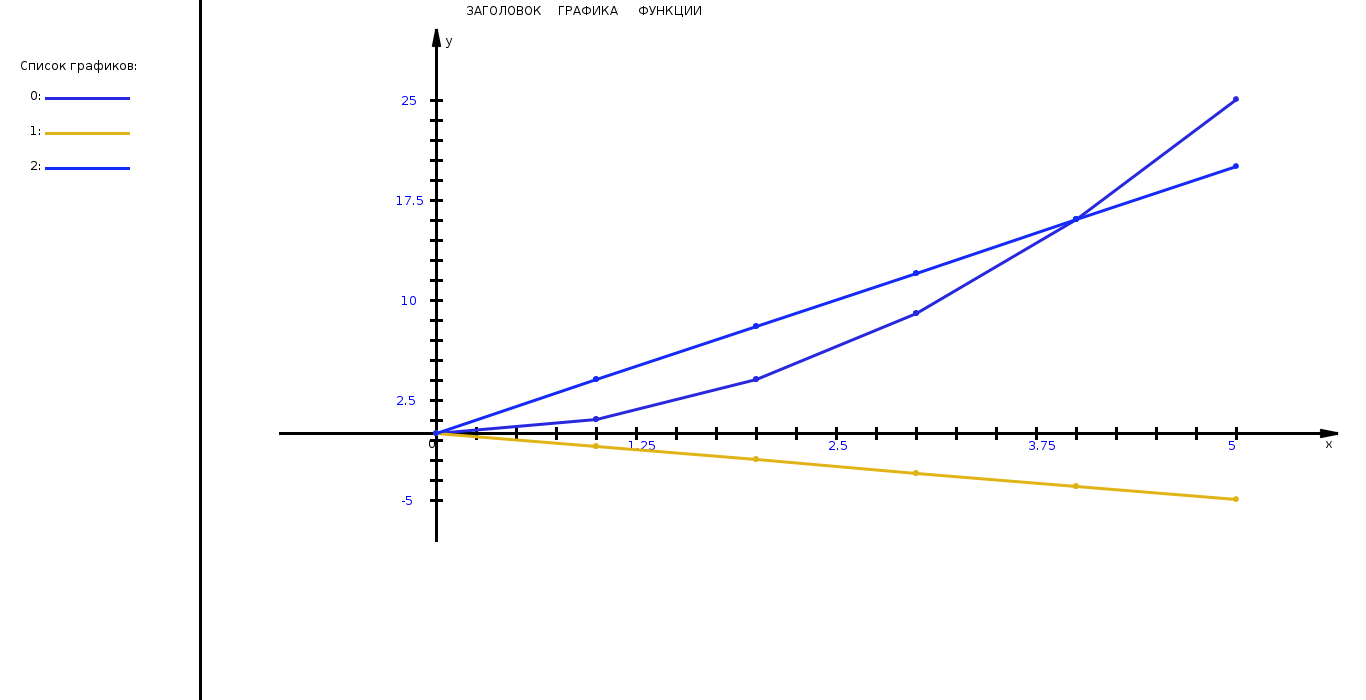
\includegraphics[scale=0.25]{pictures/2_7}
\vspace*{-10mm}
\caption{}
\label{2_7}
\end{figure}


\underline{Example 2.}
 %enddelete

 \vspace*{-2mm}
 \begin{verbatim}
 SPACE=R64[x]; 
\set2D(-1,5,-10,10);
"We have a table function"
A = [[0, 1, 2, 3, 4, 5], [3, 0, 4, 10, 5, 10]];
t = \table (A);
"We approximate this function by a polynomial of degree 4:" 
p = \approximation(t, 4);
"Building the graph of the polynomial:" P = \plot (p, [1,5]);
"Plot a table function:" T = \tablePlot (t);
"We construct both graphs in one coordinate system:" 
\showPlots ([P, T]);
 \end{verbatim}

%begindelete
\ex{}{$0.54x^4-5.64x^3+18.38x^2-17.28x+3.17$\\
\hspace*{4mm} fig. \ref{2_8}.}
\begin{figure}[!h]
 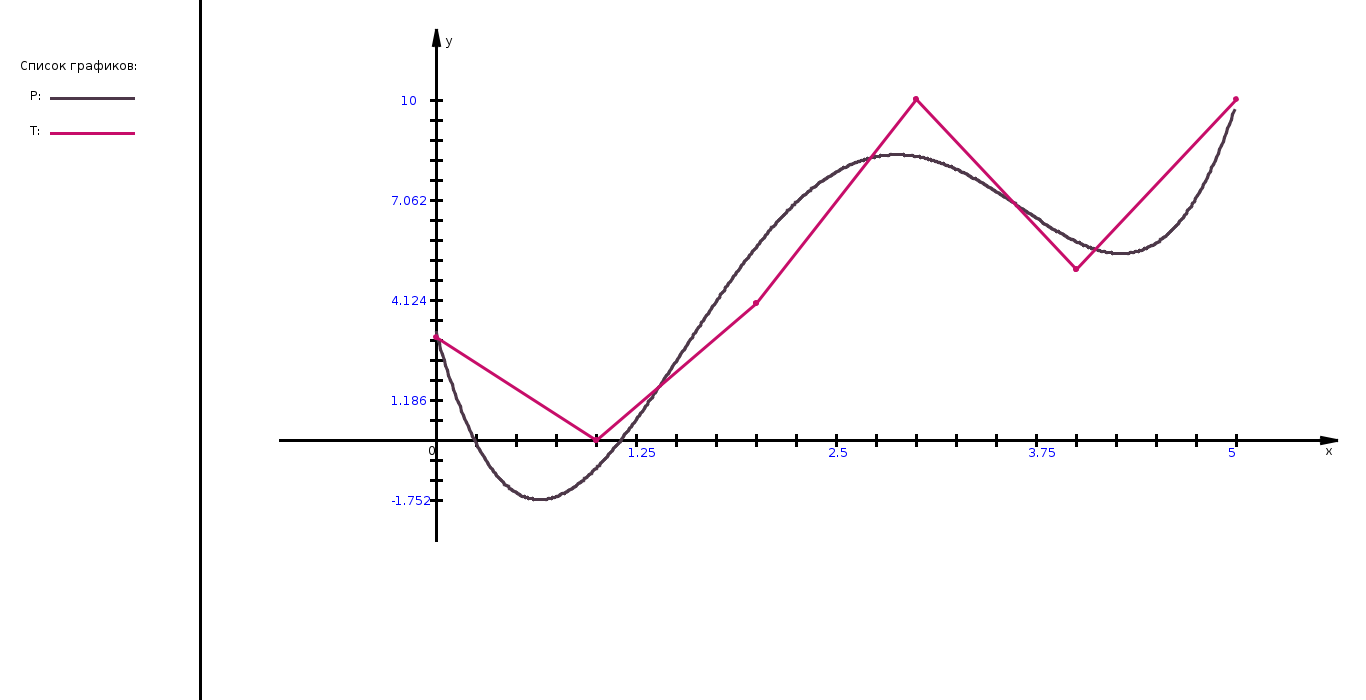
\includegraphics[scale=0.25]{pictures/2_8}
\vspace*{-10mm}
\caption{}
\label{2_8}
\end{figure}
%enddelete

%begindelete
\underline{Example 3.}
 
 \vspace*{-2mm}
%enddelete

 \begin{verbatim}
SPACE = R64[x, y, z];
\set2D(-10, 10, -10, 10, '','', 'Header of Graphics');
 \tablePlot(
   [[-3, -6, -6, -3, 3, 6, 6, 3, -3],
    [6, 3, -3, -6, -6, -3, 3, 6, 6]]);
 \end{verbatim}

%begindelete
\underline{Example 4.}
 
 \vspace*{-2mm}
%enddelete

 \begin{verbatim}
SPACE = R64[x, y, z];
 \tablePlot(
   [[-3, -6, -6, -3, 3, 6, 6, 3, -3],
    [6, 3, -3, -6, -6, -3, 3, 6, 6]],'arrow');
 \end{verbatim}

%begindelete
\underline{Example 5.}
 
 \vspace*{-2mm}
%enddelete

 \begin{verbatim}
SPACE = R64[x, y, z];
 \tablePlot(
   [[-3, -6, -6, -3, 3, 6, 6, 3, -3],
    [6, 3, -3, -6, -6, -3, 3, 6, 6]], 'dash');
 \end{verbatim}

%begindelete
\underline{Example 6.}
 
 \vspace*{-2mm}
%enddelete

 \begin{verbatim}
SPACE = R64[x, y, z];
 \tablePlot(
   [[-3, -6, -6, -3, 3, 6, 6, 3, -3],
    [6, 3, -3, -6, -6, -3, 3, 6, 6]], 'dashAndArrow');
 \end{verbatim}

\subsection{Functions that are defined on the points table of values}
Plotting functions on the points given by the tabulated values use the command: 
\comm{pointsPlot}{([[x_{1},\ldots, x_{n}],[y_{1},\ldots,y_{n}]], [s_{1},\ldots,s_{n}], [kv_{1},\ldots,kv_{n}], [kg_{1},\ldots,kg_{n}])},\\
where $s_{n}$~--- signature points, $kv_{n}$~--- rate of rotation about the point (ranges from 0 to 7, and signifies a shift in the ($kv_{n}$ * 45) degrees), 
$kg_{n}$~--- shift factor along the axis $OX$ (if it is negative then the displacement is to the left).
The reduced variants of this command:
\comm{pointsPlot}{([[x_{1},\ldots, x_{n}],[y_{1},\ldots,y_{n}]], [s_{1},\ldots,s_{n}])}
or
\comm{pointsPlot}{([[x_{1},\ldots, x_{n}],[y_{1},\ldots,y_{n}]], [s_{1},\ldots,s_{n}], [kv_{1},\ldots,kv_{n}])}
or
\comm{pointsPlot}{([[x_{1},\ldots, x_{n}],[y_{1},\ldots,y_{n}]], [s_{1},\ldots,s_{n}], [kv_{1},\ldots,kv_{n}], [kg_{1},\ldots,kg_{n}])}
 
%begindelete
\underline{Example 1.}
 
 \vspace*{-2mm}
%enddelete

\begin{verbatim}
\set2D(-10, 10, -10, 10);
\pointsPlot(
   [[0, 1, 2],
     [0, 1, 4]],['a','b','c']);
\end{verbatim}

%begindelete
\underline{Example 2.}
 
 \vspace*{-2mm}
%enddelete

\begin{verbatim}
\pointsPlot(
   [[0, 1, 2],
     [0, 1, 4]],['a','b','c'],[0,2,4]);
\end{verbatim}

%begindelete
\underline{Example 3.}
 
 \vspace*{-2mm}
%enddelete

\begin{verbatim}
\pointsPlot(
   [[0, 1, 2],
     [0, 1, 4]],['a','b','c'],[0,2,4],[0,-5,5]);
\end{verbatim}

%begindelete
\underline{Example 4.}
 
 \vspace*{-2mm}
%enddelete

\begin{verbatim}
\pointsPlot(
   [[0, 1, 2],
     [0, 1, 4]]);
\end{verbatim}

%begindelete
\underline{Example 5.}
 
 \vspace*{-2mm}
%enddelete

\begin{verbatim}
SPACE = R64[x, y, z];
f1=\tablePlot([[1, 1], [1, 5]]);
f2=\tablePlot([[1, 5], [1, 1]]);
f3=\tablePlot([[5, 5], [1, 5]]);
f4=\tablePlot([[1, 5], [5, 5]]);
f5=\pointsPlot([[1, 1, 5, 5],[1, 5, 5, 1]],['A','B','C','D'],[6,0,0,2]);
\showPlots([f1, f2, f3, f4, f5]);
\end{verbatim}

%begindelete
\underline{Example 6.}
 
 \vspace*{-2mm}
%enddelete

\begin{verbatim}
SPACE = R64[x, y, z];
f1=\tablePlot([[1, 1], [1, 5]]);
f2=\tablePlot([[1, 5], [1, 1]]);
f3=\tablePlot([[5, 5], [1, 5]]);
f4=\tablePlot([[1, 5], [5, 5]]);
f5=\pointsPlot([[1, 1, 5, 5],[1, 5, 5, 1]],['A','B','C','D'],[6,0,0,2]);
\showPlots([f1, f2, f3, f4, f5], 'noAxes');
\end{verbatim}

\subsection{Construction of various plots of functions in one coordinate system}
To construct the plots of functions defined in different ways, you must first build a plot of each function and then execute the command  
\comm{showPlots}{([f_1, f_2, \ldots, f_n])}.

Another version of the command:
\comm{showPlots}{([f1, f2, f3, f4], 'noAxes')}, where 'noAxes'~--- parameter indicating image graphics without axes.
or
\comm{showPlots}{([f1, f2, f3, f4], 'lattice')}, where 'lattice'~--- parameter indicating the image graph with the lattice.

%begindelete
\underline{Example 1.}
 
 \vspace*{-2mm}
%enddelete

\begin{verbatim}
SPACE = R64[x, y, z];
\set2D(-20, 20, -20, 20);
f1 = \plot(\tg(x));
f2 = \tablePlot([[0, 1, 4, 9, 16, 25], [0, 1, 2, 3, 4, 5]]);
f3 = \paramPlot([\sin(x), \cos(x)], [-10, 10]);
f4=\tablePlot([[0, 1, 4, 9, 16, 25], [0, -1, -2, -3, -4, -5]]);
\showPlots([f1, f2, f3, f4]);
\end{verbatim}
%begindelete
\ex{}{fig. \ref{3_6}.}
\begin{figure}[!ht]
 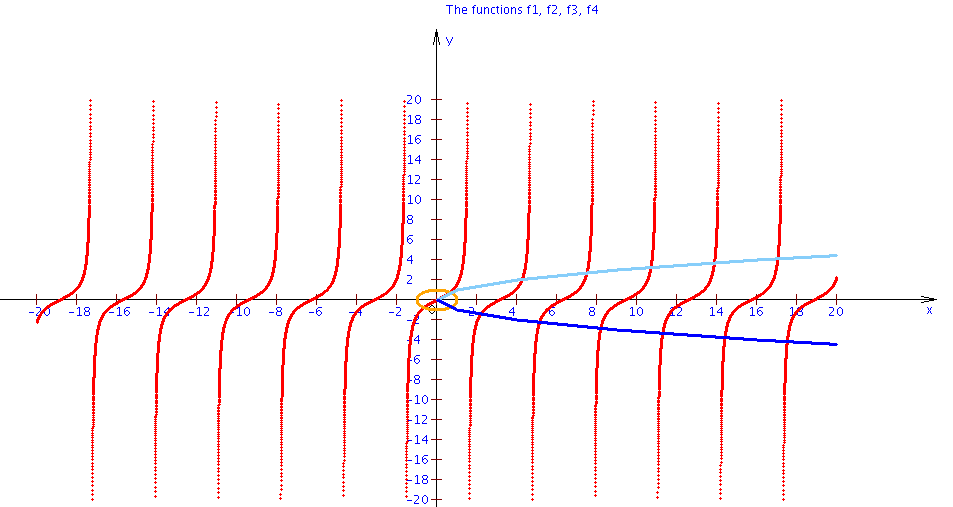
\includegraphics[scale=0.6]{pictures/3_6}
\caption{Graphs of functions defined in different ways}
\label{3_6}
\end{figure}
%enddelete

%begindelete
\underline{Example 2.}
 
 \vspace*{-2mm}
%enddelete

 \begin{verbatim}
p1=\tablePlot([[-1, -3, 3, 3, -3, -3],[4, 3, 3, -3 , -3, 3]]);
p2=\tablePlot([[5, 5, 3, 3, 5, -1],[4, -2, -3, 3, 4, 4]]);
p3=\tablePlot([[-3, -1, -1],[-3, -2, 4]], 'dash');
p4=\tablePlot([[-1, 5],[-2, -2]], 'dash');
\showPlots([p1,p2,p3,p4], 'noAxes');
 \end{verbatim}

%begindelete
\underline{Example 3.}
 
 \vspace*{-2mm}
%enddelete

 \begin{verbatim}
p1=\tablePlot([[-1, -3, 3, 3, -3, -3],[4, 3, 3, -3, -3, 3]]);
p1p=\pointsPlot([[-1, -3, 3, 3, -3],[4, 3, 3, -3 , -3]],['F','B','C','D','A'],[0,0,0,4,4]);
p2=\tablePlot([[5, 5, 3, 3, 5, -1],[4, -2, -3, 3, 4, 4]]);
p3=\tablePlot([[-3, -1, -1],[-3, -2, 4]],'dash');
p4=\tablePlot([[-1, 5],[-2, -2]],'dash');
p2p=\pointsPlot([[5, 5, -1 ],[4, -2, -2]],['G','H','E'],[0,4,4]);
\showPlots([p1,p2,p3,p4,p1p,p2p], 'noAxes');
 \end{verbatim}

\subsection{Construction of graphs}
To construct the graph, use the command
\comm{plotGraph}{([[a_{11},\ldots,a_{1n}],\ldots,[a_{n1},\ldots,a_{nn}]], [[x_{1},\ldots, x_{n}],[y_{1},\ldots,y_{n}]])}, 
where $[[a_{11},\ldots,a_{1n}],\ldots,[a_{n1},\ldots,a_{nn}]]$ ~--- adjacency matrix, $[[x_{1},\ldots, x_{n}],[y_{1},\ldots,y_{n}]]$ ~--- matrix of coordinates.

%begindelete
\underline{Example 1. }
%enddelete

\vspace*{-2mm}
\begin{verbatim}
SPACE = R64[x, y, z];
\plotGraph([[0,1,1,0,1,0],[1,0,0,1,1,0],[1,0,0,0,1,1],[0,1,0,0,0,0],
[1,1,1,0,0,1],[0,0,1,0,1,0]],[[3,2,4,1,3,5],[3,2,2,1,1,1]]);
\end{verbatim}
%begindelete
\ex{}{pict. \ref{4_1}.}
\begin{figure}[!ht]
 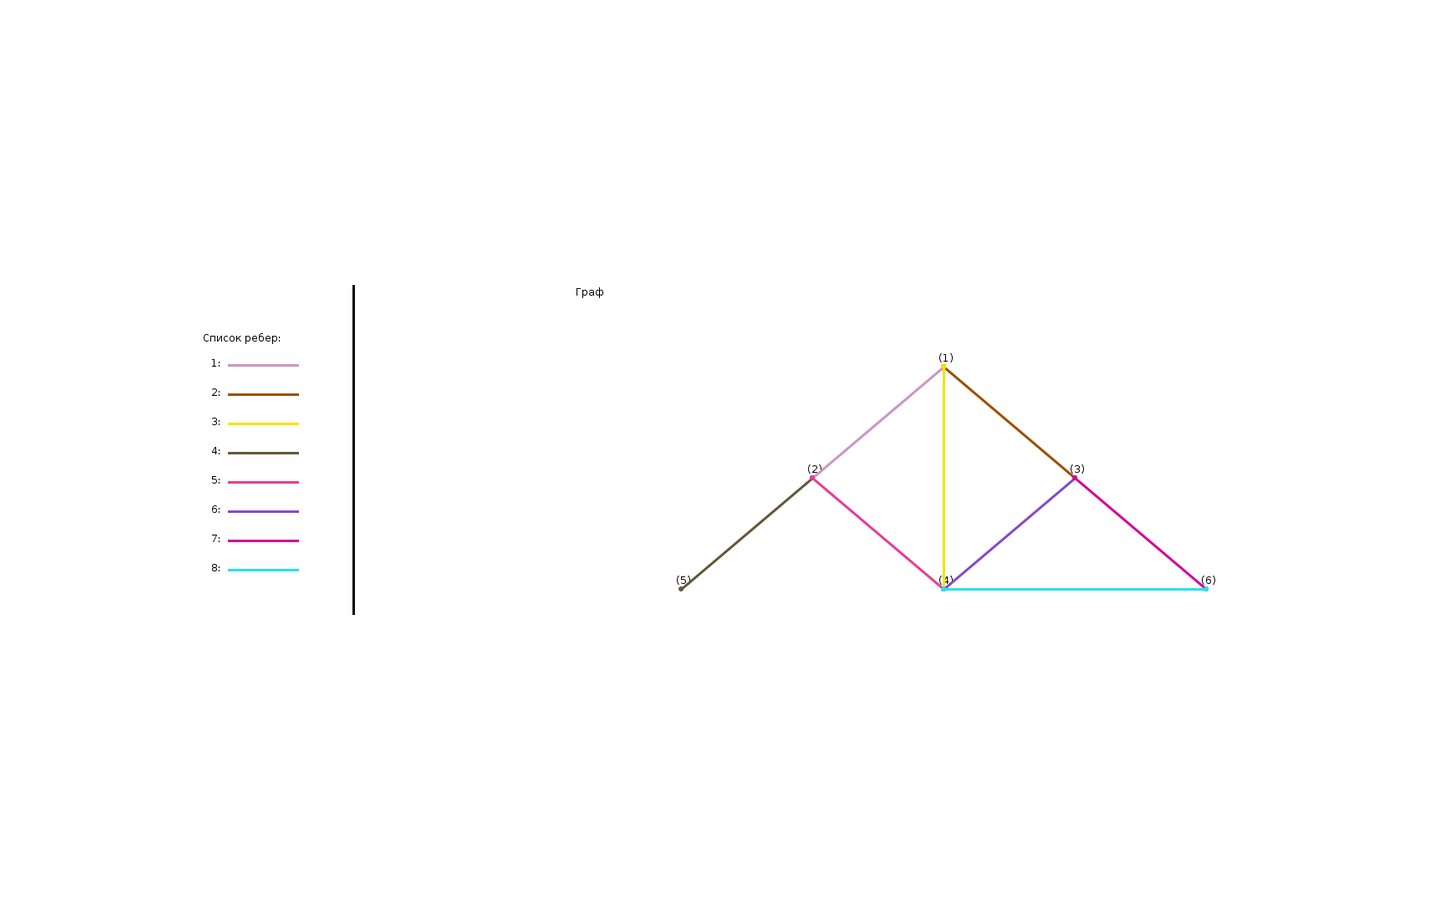
\includegraphics[scale=0.4]{pictures/4_1}
\caption{graph}
\label{4_1}
\end{figure}
%enddelete

In addition, you can run only with the first parameter
\comm{plotGraph}{([[a_{11},\ldots,a_{1n}],\ldots,[a_{n1},\ldots,a_{nn}]])}, 
where $[[a_{11},\ldots,a_{1n}],\ldots,[a_{n1},\ldots,a_{nn}]]$ ~--- adjacency matrix.

%begindelete
\underline{Example 2. }
%enddelete

\vspace*{-2mm}
\begin{verbatim}
SPACE = R64[x, y, z];
\plotGraph([[0,1,1,0,1,0],[1,0,0,1,1,0],[1,0,0,0,1,1],[0,1,0,0,0,0],
[1,1,1,0,0,1],[0,0,1,0,1,0]]);
\end{verbatim}
%begindelete
\ex{}{pict. \ref{4_2}.}
\begin{figure}[!ht]
 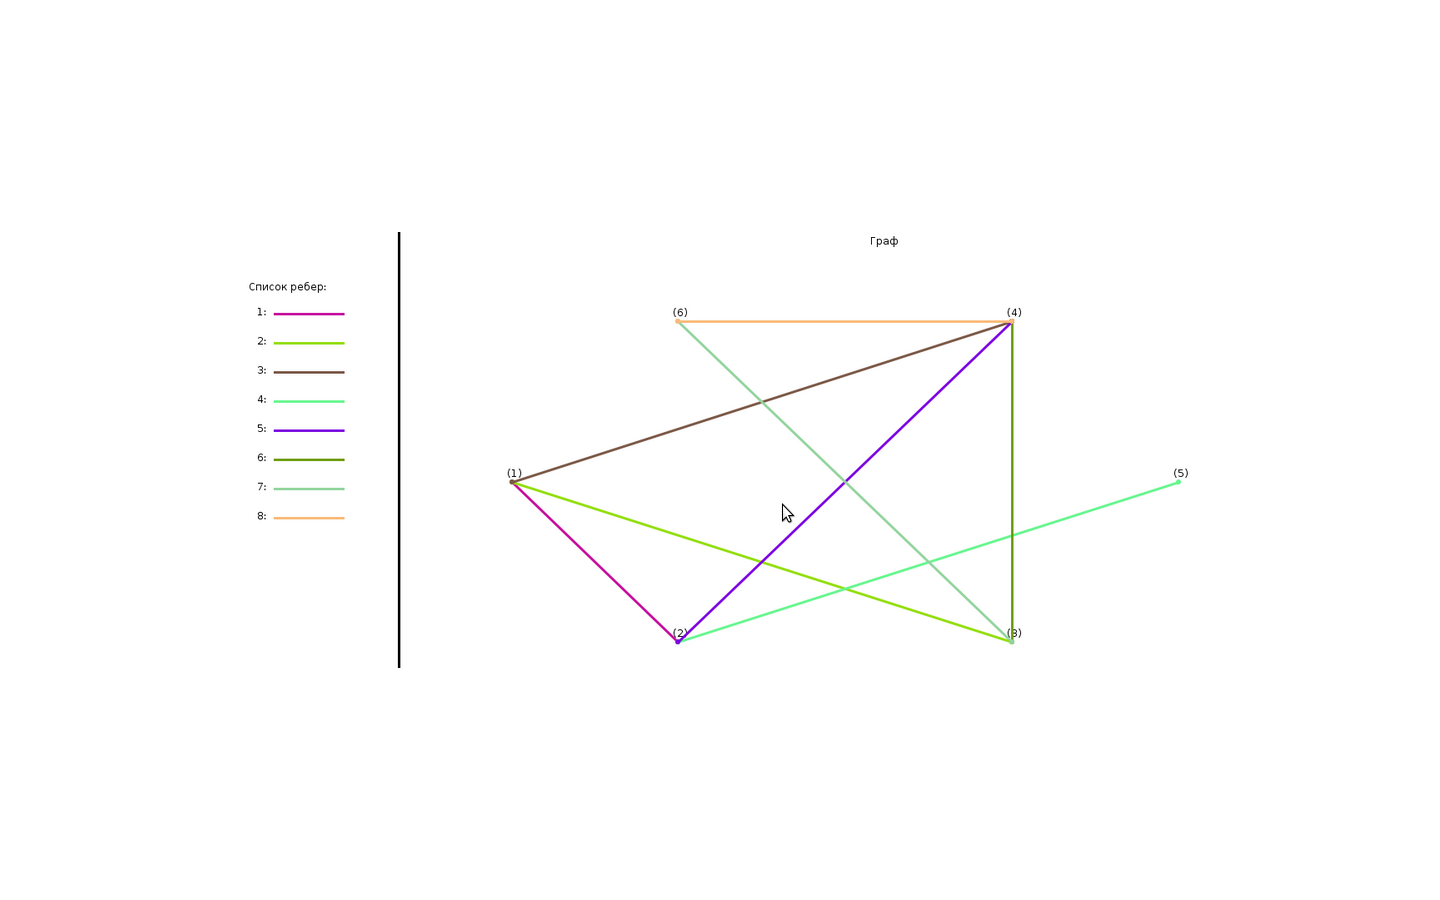
\includegraphics[scale=0.4]{pictures/4_2}
\caption{graph}
\label{4_2}
\end{figure}
%enddelete

You need to run a single numeric parameter
\comm{plotGraph}{(N)}, 
where $N$ ~--- the number of vertices in a graph.

%begindelete
\underline{Example 3. }
%enddelete

\vspace*{-2mm}
\begin{verbatim}
SPACE = R64[x, y, z];
\plotGraph(6);
\end{verbatim}
%begindelete
\ex{}{pict. \ref{4_3}.}
\begin{figure}[!ht]
 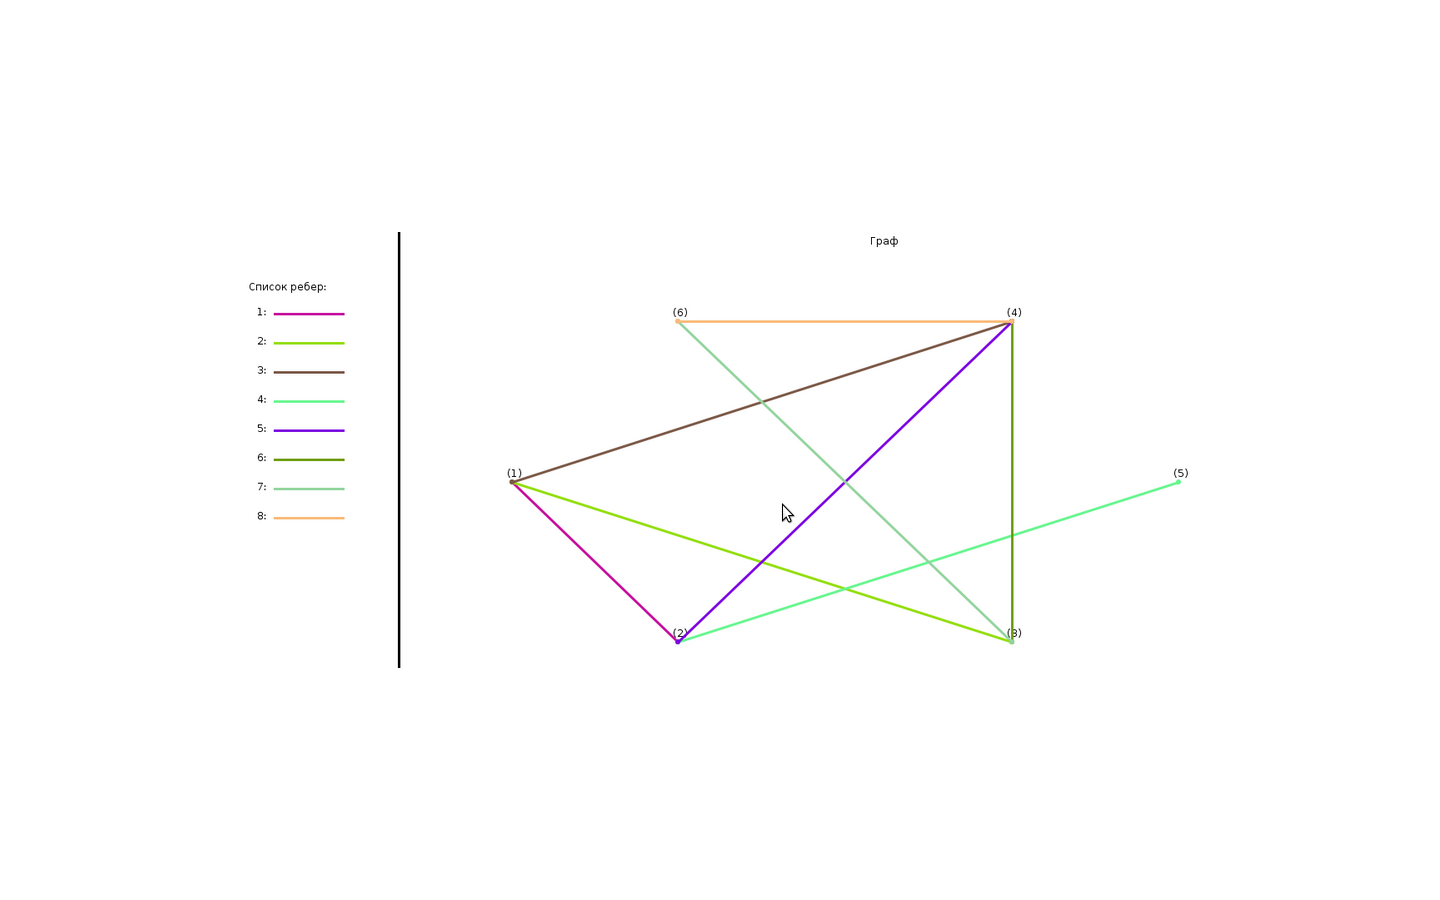
\includegraphics[scale=0.4]{pictures/4_2}
\caption{graph}
\label{4_3}
\end{figure}
%enddelete

\section{Plots 3D of explicit functions} 
You can build 3D graphs of the functions that are defined explicitly. 
 
To obtain the plot 3D of an explicit function $f=f(x,y)$ the command 
\comm{plot3d}{(f, [x0, x1, y0, y1])}, 
 is used, where $[x0, x1]$ is an interval on the axis $OX$, $[y0, y1]$ is an interval on the axis $OY$.

The obtained plot can be rotated and to increase or decrease.

Moving the mouse holding down the left <<mouse>> button causes the rotation of the coordinate system of schedule.
After stopping the movement of the <<mouse>> graphics are redrawn in the new rotated coordinate system.
 
Moving the mouse holding down the left mouse button while pressing ${\it Shift}$ button leads 
to a change in image scale. After stopping the movement of the <<mouse>> graphics are redrawn in the new scale.

%begindelete
\underline{Example. }

\vspace*{-2mm}
%enddelete

\begin{verbatim}
SPACE = R64[x, y, z];
f = x^2 / 20 + y^2 / 20;
\plot3d(f, [-20, 20, -20, 20]);
\end{verbatim}

\begin{verbatim}
SPACE = R64[x, y, z];
\plot3d([x / 20 + y^2 / 20, x^2 / 20 + y / 20], [-20, 20, -20, 20]);
\end{verbatim}

\begin{verbatim}
SPACE = R64[x, y, a, b];
f = ax^2 / 20 + by^2 / 20;
\plot3d(f, [-20, 20, -20, 20]);
\end{verbatim}

Sphere 

\begin{verbatim}
SPACE=R64[u,v];
\paramPlot3d([[\cos(u)\cos(v)],[\sin(u)\cos(v)],[\sin(v)]], [-\pi, \pi, -\pi/2, \pi/2]);
\end{verbatim}

Thor 

\begin{verbatim}
SPACE=R64[u,v];
\paramPlot3d([[\cos(u)(\cos(v)+3)],[\sin(u)(\cos(v)+3)],[\sin(v)]], [-\pi, \pi, -\pi, \pi]);
\end{verbatim}

Spiral

\begin{verbatim}
SPACE=R64[u,v];
\paramPlot3d([[\cos(u)(\cos(v)+3)],[\sin(u)(\cos(v)+3)],[\sin(v)+u]], [-2\pi, 2\pi, -\pi, \pi]);
\end{verbatim}

Logarithmic spiral 

\begin{verbatim}
SPACE=R64[u,v];
\paramPlot3d([[u\cos(u)(\cos(v)+1)],[u\sin(u)(\cos(v)+1)],[u\sin(v)]], [0, 3\pi, -\pi, \pi]);
\end{verbatim}

"Seashell" 

\begin{verbatim}
SPACE=R64[u,v];
\paramPlot3d([[u\cos(u)(\cos(v)+1)],[u\sin(u)(\cos(v)+1)],[u\sin(v)-(((u+3)/8)\pi)^2-20]], [0, 8\pi, -\pi, \pi]);
\end{verbatim}

Shamrock 

\begin{verbatim}
SPACE=R64[u,v];
\paramPlot3d([[\cos(u)\cos(v)+3\cos(u)(1.5+\sin(1.5u/2))],[\sin(u)\cos(v)+3\sin(u)(1.5+\sin(1.5u/2))],[\sin(v)+2\cos(1.5u)]], [-2\pi, 2\pi, -\pi, \pi]);
\end{verbatim}

Dini surface 

\begin{verbatim}
SPACE=R64[u,v];
\paramPlot3d([[\cos(u)\sin(v)],[\sin(u)\sin(v)],[\cos(v)+\lg(\tg(v/2))+0.2u-4]], [0, 4\pi, 0.0001, 2]);
\end{verbatim}

Tape Mobius

\begin{verbatim}
SPACE=R64[u,v];
\paramPlot3d([[(1+v/2\cos(u/2))\cos(u)],[(1+v/2\cos(u/2))\sin(u)],[v/2\sin(u/2)]], [0, 2\pi, -1, 1]);
\end{verbatim}

Cube

\begin{verbatim}
SPACE=R64[u,v];
\paramPlot3d([[u,v,5,u,v,-5],[v,5,u,v,-5,u],[5,u,v,-5,u,v]], [-5, 5, -5, 5]);
\end{verbatim}

Cylinder

\begin{verbatim}
SPACE=R64[u,v];
\paramPlot3d([[5\cos(u)],[5\sin(u)],[v]], [-5, 5, -5, 5]);
\end{verbatim}

Cone 

\begin{verbatim}
SPACE=R64[u,v];
\paramPlot3d([[\cos(u) * (5 * (1 - v/6))],[\sin(u) * (5 * (1 - v/6))],[v]], [-6, 6, 0, 6]);
\end{verbatim}

Truncated cone 

\begin{verbatim}
SPACE=R64[u,v];
\paramPlot3d([[\cos(u) * (5 * (1 - v/6) + 1 * v/6)],[\sin(u) * (5 * (1 - v/6) + 1 * v/6) ],[v]], [-5, 5, -5, 5]);
\end{verbatim}

Hourglass

\begin{verbatim}
SPACE=R64[u,v];
\paramPlot3d([[\cos(u) * (5 * (0.5 - v/6) + 0.01*v/6)],[\sin(u) * (5 * (0.5 - v/6) + 0.01*v/6)],[v]], [0, 2\pi, 0, 2\pi]);
\end{verbatim}


%begindelete
 
\ex{$f=x^2/20+y^2/20;$\\
\hspace*{4mm} $plot3d(f, [-20, 20, -20, 20]);$\\
\hspace*{4mm} $plot3d([x/20+y^2/20, x^2/20+y/20], [-20, 20, -20, 20]);$}
{fig. \ref{3_7}.}

\begin{figure}[!ht]
  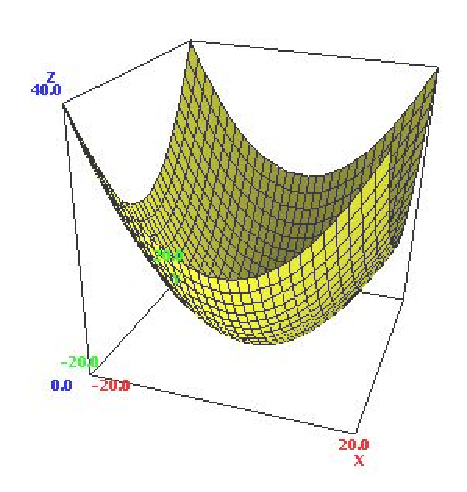
\includegraphics[width=138pt, height=146pt]{pictures/3_7}
  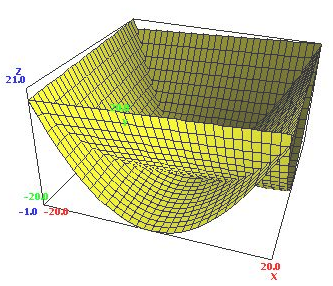
\includegraphics[width=166.5pt, height=143pt]{pictures/3_8}
  \caption{Plots 3D of  functions}
  \label{3_7}
\end{figure}
%enddelete


\section{Ploting of 3D graphs of functions that are defined implicitly} 
You can build 3D graphs of the functions that are defined implicitly. 
 
To construct the graph of an implicit function $ f(x,y,z)=0$ use the command 

 \comm{implicitPlot3d}{(f, x0, x1, y0, y1,z0, z1)}, 

where the numbers $xMin, xMax, yMin, yMax, zMin, zMax$  set the box in the space, 
which is represented by an implicit function. 

You can specify only one function, like this

 \comm{implicitPlot3d}{(f)}

in this case it is assumed that there will be shows the function $ f $ in the cube 
$ 20\times 20 \times 20$,
 which is placed on a center origin.

You can rotate the coordinate system by moving the mouse pointer while holding down the left button.
You can move the coordinate system by moving the mouse pointer while holding down the right button.

It is possible, optionally, to specify the coordinates of the light source, the color of the surface and the grid size. The default grid of 50 points on each edge of the box.

The color format $RGB$ (red, green, blue) is given a number

$R * 256 * 256+ G *256 + B$,

 where each letter denotes a non-negative integer not exceeding 255.
For example, $ 255 * 256 * 256 $ --- red, and $ 255 * 256 * 256 + 255 * $ 256 --- yellow (red + green).

Allowed, in addition, the following sets of arguments:

$(F, xMin, xMax, yMin, yMax, zMin, zMax, gridSize)$,

$(F, xMin, xMax, yMin, yMax, zMin, zMax, lightX, lightY, lightZ, gridSize)$,

$(F, xMin, xMax, yMin, yMax, zMin, zMax, lightX, lightY, lightZ, color, gridSize)$.

%begindelete
\underline{Example. }

\vspace*{-2mm}
%enddelete


\begin{verbatim}
SPACE = R64[x, y, z];
 
f = -x^2+2y^2+3z^2-25;
\implicitPlot3d( f, -10, 10, -10, 10, -10, 10);
\end{verbatim}

 
Hyperboloid



\begin{verbatim}
SPACE = R64[x, y, z ];
\implicitPlot3d( x^2+ y^2+ z^2-25 , -7, 7, -7, 7, -7, 7,10, 10, 10, 255*256*256, 100);
\end{verbatim}

Red sphere.




\begin{verbatim}
SPACE = R64[x, y, z]; 
f =  \sin(xyz/100) ;
\implicitPlot3d( f , -9,9,-9,9,-9,9, 10,10, 4, 255*256*256+255*256, 50);
\end{verbatim}

Yellow surface with a central symmetry.


\begin{verbatim}
SPACE = R64[x, y, z]; 
f = ((x+2)^2+ (y-2)^2 -1)((x-2)^2+ (y+2)^2 -1)((x+2)^2+ (y+2)^2 -1) ((x-2)^2+ (y-2)^2 -1)(x^2+ y^2 -1); 
\implicitPlot3d( f, -10, 10, -10, 10, -10, 10 );
\end{verbatim}

Organ pipes.
